\documentclass[aspectratio=1610,17pt,utf8]{beamer}

\usepackage[utf8]{inputenc}
\usepackage[T1]{fontenc}
\usepackage[USenglish]{babel}
\usepackage{graphicx} % graphics
\usepackage{mathabx}
\usepackage{mathpazo}
\usepackage{eulervm}

\usetheme{unipassau}


% title slide definition
\title[Misbehaviour Prediction for SDC]{5846HS: Search-based Software Engineering for Testing Autonomous Cars}
\subtitle{Misbehaviour Prediction for Autonomous Driving Systems}
\author[Vuong Nguyen]{Vuong Nguyen}
\institute[Fakultät]
{
  Universität Passau\\
  Lehrstuhl für Software Engineering II\\
}
\date{SoSe 20}

%--------------------------------------------------------------------
%                            Titlepage
%--------------------------------------------------------------------

\begin{document}

\begin{frame}[plain]
  \titlepage
\end{frame}

\begin{frame}[plain]
  \tableofcontents
\end{frame}

%-------------------------------------------------------------------
%                            Content
%-------------------------------------------------------------------

\section{Introduction}

\subsection{Solutions for testing Autonomous Driving Systems}
\begin{frame}{Techniques for testing SDC}
  \begin{itemize}
    \item Offline Solutions
    \item Online Solutions
  \end{itemize}
\end{frame}

\begin{frame}{Techniques for testing - Offline Solutions}
  \begin{itemize}
    \item Testing Autonomous Cars for Feature Interaction Failures Using Many-objective Search.
    \item Testing advanced driver assistance systems using multi-objective search and neural networks.
    \item Testing VisionBased Control Systems Using Learnable Evolutionary Algorithms.
    \item ... and so on.
  \end{itemize}
  %-------------------------------------------------------------------
  % Such autonomous driving systems receive data from a multitude of 
  % sensors and to test such software systems, companies perform several 
  % simulation-based test scenarios on both normal conditions as well as 
  % challenging and dangerous circumstances.
  %
  % Such testing used to improve the safety and reliability of self-driving 
  % car and expose weakness of those systems for extreme conditions.
  %-------------------------------------------------------------------
\end{frame}

\begin{frame}{Techniques for testing - Online Solutions}
  \begin{itemize}
    \item Misbehaviour Prediction for Autonomous Driving Systems.
  \end{itemize}
  
  %-------------------------------------------------------------------
  % On the other hand, the online solution, which is proposed by the paper, 
  % focuses on estimating confidence for self-driving vehicles with the 
  % aim of predicting the occurrence of misbehaviours
  % and enable self-healing procedures that can avoid collision or driving out of roads.
  %-------------------------------------------------------------------
\end{frame}

\subsection{Misbehaviour Prediction for Autonomous Driving Systems}
\begin{frame}{Misbehaviour Prediction for SDC - Goals}
  \begin{itemize}
    \item Recognizing when a self-driving car is within a low-confidence area.
    \item Predicting such situation timely enough so as to take countermeasures.
  \end{itemize}
  
  %-------------------------------------------------------------------
  % The approach addresses two problems:
  % 1. Recognizing when a self-driving car is within a low-confidence area because of an unexpected/untested execution context/behaviour 
  % 2. Predicting such situation timely enough so as to take countermeasures before the vehicle may crash (collision) or drive off road (out-of-bounds episodes).  
  %-------------------------------------------------------------------
\end{frame}

\begin{frame}{Misbehaviour Prediction for SDC - Goals}
  \begin{figure}[!htb]
    \begin{minipage}{0.48\textwidth}
      \centering
      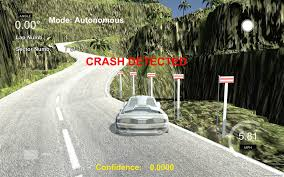
\includegraphics[width=1\linewidth]{fig00.jpeg}
      \caption{Collision}
      \label{Fig:Data1}
    \end{minipage}\hfill
    \begin{minipage}{0.48\textwidth}
      \centering
      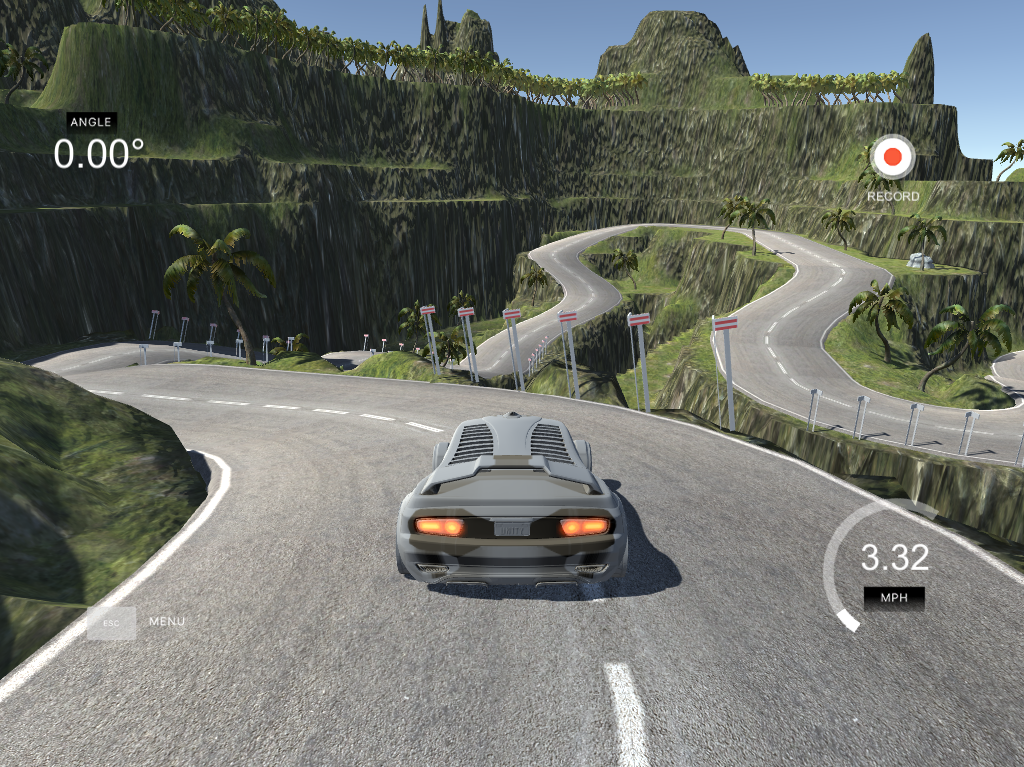
\includegraphics[width=1\linewidth]{fig01.png}
      \caption{Out-of-bounds episodes}
      \label{Fig:Data2}
    \end{minipage}
  \end{figure}
\end{frame}

%%%%%%%%%%%%%%%%%%%%%%

\section{SelfOracle}

\begin{frame}{Definition of Misbehaviour}
A DNN exhibits a misbehaviour in a given test scenario if the overall system that contains the DNN does not respect its requirements due to the outputs produced by the DNN.
  %-------------------------------------------------------------------
  % Given a specific scenarios, if the output of DNN does not satisfy 
  % or violate any safety requirements, it means the DNN is showing 
  % a misbehaviour and we will estimate a threshold theta to predict
  % a misbehaviour of DNN.  
  %-------------------------------------------------------------------
\end{frame}

\begin{frame}{Definition of Misbehaviour}
  \begin{figure}[!htb]
   	\centering
   	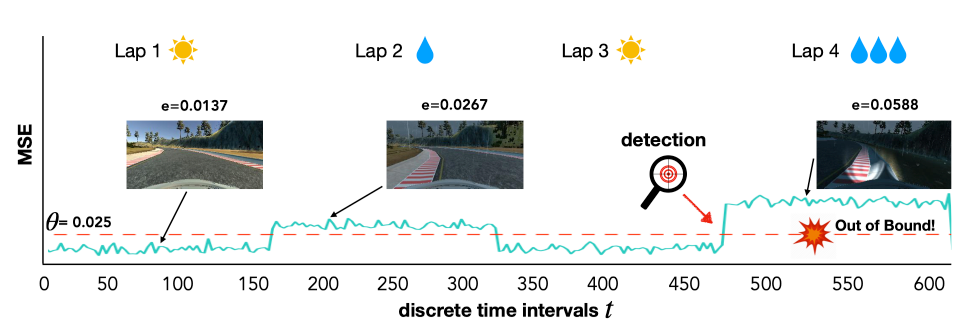
\includegraphics[width=1\linewidth]{fig02.png}
    \caption{Confidence levels of NVIDIA’s DAVE-2}
    \label{Fig:Data3}
  \end{figure}

  %-------------------------------------------------------------------
  % We use the estimated θ as threshold to distinguish anomalous conditions from normal ones.
  % As we can see, confidence levels of the DNN is changing in response to changing driving scenarios.
  % We have 4 different conditions: (Lap 1) sun, (Lap 2) light rain, (Lap 3) sun, and (Lap 4) heavy rain.
  %
  % The reconstruction error is low when the car drives under sunny conditions which indicates normal behaviour.
  % In contrast, the error increases with extreme conditions and grows above a given threshold which indicates misbehaviours.
  % 
  % As a result, this cause the SDC to drive off the road.
  %-------------------------------------------------------------------
\end{frame}



\begin{frame}{Hello?}

\begin{itemize}
\item How are you?
\item I'm good
\end{itemize}
\end{frame}

%%%%%%%%%%%%%%%%%%%%%%

\section{Example}

%%%%%%%%%%%

\begin{frame}{Lunch Menu}

\begin{itemize}
\item Spaghetti
  \begin{itemize}
  \item Bolognese
  \item Aglio olio
  \end{itemize}
\item Sandwiches
  \begin{itemize}
  \item Egg
  \item Ham
  \item Tuna
  \end{itemize}
\end{itemize}
\end{frame}

%%%%%%%%%%%

\subsection{Budgeting}

\begin{frame}{Projected Profit}

\begin{enumerate}
\item And the answer is...
\item $f(x)=\frac{f^{(n)}(a)}{n!}(x-a)^n$
\end{enumerate}

\end{frame}

%%%%%%%%%%%

\end{document}
